\section{Hud- och handidentifiering}

\subsection{Klassificering av hud}
I 44 bilder tagna med webbkameran separerades huden från resten av
bilden manuellt med hjälp av fotoredigeringsprogramvara (se figur
\vref{fig:hudseparerad}. Baserat på
dessa bildpunkter bestämdes sedan en sannolikhetsfördelning för både hud
och icke-hud enligt kapitel \ref{sec:hudklassificering}). 

\begin{figure}[tb]
	\centering 
	\subfloat[Hud]{
		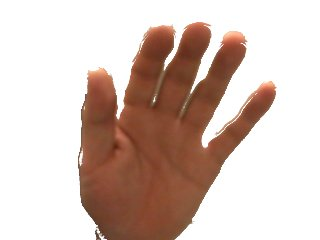
\includegraphics[width=0.45\columnwidth]{bilder/hud.png}
		\label{fig:hud}
	}
	% ev. spacing
	\subfloat[Ickehud]{
		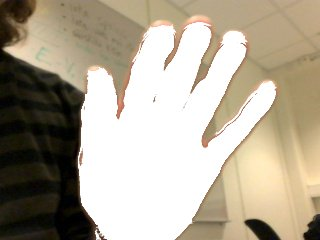
\includegraphics[width=0.45\columnwidth]{bilder/ohud.png}
		\label{fig:ohud}
	}
	\caption{För att skapa sannolikhetsfördelningar för hudfärg
          respektive färg för ickehud togs 44 bilder ur vilka huden
          spearerades från övriga bilden.}
	\label{fig:hudseparerad}
\end{figure}


Med hjälp av
sannolikhetsfördelningarna delades kamerabilden in i hud
resp.~ickehud, så att resultatet kunde bedömas. För att inte behöva
räkna ut sannolikheten för färgen i varje bildpunkt och bildruta
som analyseras,
vilket hade krävt lång beräkningstid, gjordes beräkningen
i förväg för varje tänkbar färg ($256^2$ stycken i
$C_bC_r$-rymden). Resultaten sparades
sedan i två $256\times256$-matriser, där färgvärdet användes som
koordinater. Ett antal binära matriser skapades sedan med ettor på de
positioner där klassificeringskravet 
\begin{equation*}
	\frac{\Prob(\textrm{färg}|\textrm{hud})}{\Prob(\textrm{färg}|\textrm{ickehud})} > c,
\end{equation*}
var uppfyllt för olika värden på konstanten c. Ju större c var desto färre
färger klassades som hud. 

I dessa matriser, eller
''hudfärgskartor'', kunde man sedan slå upp
färgvärden för att direkt få veta om dessa skulle klassas som hud.
De olika kartorna testades, och den som gav en så bra bild av
handen som möjligt utan att ta med stora bakgrundsområden användes.
Metoden med hudfärgskartor har visats vara effektiv av bl.a.~\citeasnoun{Brand00}

De resulterande binära bilderna jämfördes sedan med dem som erhölls med
sannolikhetsfördelningarna framtagna av \citeasnoun{Elmezain08}. Detta
för att bestämma kvaliteten på våra prametrar.

\subsection{Urskiljning av handen}\label{sec:metod_hud:urskiljning}
När väl hudbildpunkterna i figuren urskilts återstår att 
identifiera handen som ska följas. Det är troligt att man i bilden
fått med ett antal mindre områden som felaktigt bedömts vara
hud. Dessutom är huvudet ofta med i bilden, vilket kan ställa till med
problem. 

Vår lösning på problemet är att först använda den inbyggda
MATLAB-funktionen \texttt{bwareaopen}, som är en morfologisk
öppningsfunktion. Metoden som beskrivs i
\ref{sec:morph} använder ett strukturelement $S$, som \texttt{bwareaopen}
genererar utifrån en parameter som specificerar
dess area --- vad som är en lämplig area
varierar med upplösning och
och avstånd till kameran. Vi använder en gräns på 200
bildpunkter, vilket fungerar bra även för relativt stort avstånd till
kameran med en upplösning på $320\times240$ bildpunkter.

För att hitta handen gör vi antagandet att handen är det
objekt som befinner sig längst till vänster i bilden.
Vi sveper därför över bildmatrisens kolonner från
vänster för att se om kolonnen innehåller någon hudbildpunkt --- den första
hudbildpunkten som nås på detta sätt antas tillhöra handen.
Det sammanhängande område som bildpunkten är en del av antas därför vara
den sökta handen.

Att på detta sätt välja objektet längst till vänster
har tidigare gjorts av bl.a. \citeasnoun{Nielsen04}. De använde
sig dock av det högra av de två största sammanhängande objekten,
vilket har fördelen att man inte behöver sätta en manuell gräns för
när ett objekt är ''tillräckligt stort''.
Till nackdelarna hör
att man tvingas
söka igenom hela bilden, att den är något svårare att
implementera samt att den endast fungerar då både huvud och hand finns
i bilden. Dessutom fungerar den endast för högerhänta användare, men kan
relativt enkelt göras tillgänglig även för vänsterhänta. Om endast statiska
gester ska behandlas räcker det med att spegelvända bilden, medan man för
dynamiska gester (eftersom rörelseriktningen spelar roll) måste söka från
höger istället, och även skapa en separat träningsmängd.

Metoden inkluderar all hud som hänger samman med
handen, vilket innefattar armen när personen framför kameran bär en kortärmad
tröja.
För att
kringgå detta kan man identifiera handleden och ''kapa'' handen
där. Detta gjordes av \citeasnoun{Deimel99} genom att identifiera den 
största cirkel
som får plats helt i handen, och som antags vara centrerad mitt i handen. Då
cirkeln förstoras något är det längsta cirkelsegment som helt får
plats inom hudområdet placerat vid handleden, och mittpunktstangenten
till segmentet skär handleden --- handen utgörs då av hudområdet på den
sida om handleden där cirkeln befinner sig. Denna metod har vi dock
inte testat, varför den filmade förväntas bära
långärmad tröja. 
\notes{otydligt! mittpunktstangenten?}
